%\RequirePackage{fixltx2e}
%\documentclass[floatfix,aps,prd,amsmath,amssymb]{revtex4}
%\usepackage{graphicx}
%\usepackage{caption}
%\usepackage{subcaption}
%\captionsetup{compatibility=false}
%\usepackage[noabbrev,capitalise]{cleveref}
%\usepackage{braket}
%\begin{document}

\section{B mesons and CPV}
\vspace{-1.0em}
\begin{center}
\tiny{\textit{John Ronayne}}
\end{center}
\subsection{Asymmetric decay rates in B meson} 
The neutral B meson is composed of the 1st generation down quark and a 3rd generation bottom quark. While this doesn't contrast the neutral Kaon oscillations to major extent in the preliminaries, the added benefit of the CKM mechanism is that it is clear to see why the B mesons produce a much more dramatic effect. Jumping ahead one can define the linear combinations of the B meson system with eigenfunction of $\hat{C}\hat{P}$,
\begin{equation}\label{BPME1}
\ket{B^{0}_{1}}=\frac{1}{\sqrt{2}}(\ket{B^{0}(d\bar{b})}+\ket{\bar{B}^{0}(\bar{d}b)}),
\end{equation}
\begin{equation}\label{BPME2}
\ket{B^{0}_{2}}=\frac{1}{\sqrt{2}}(\ket{B^{0}(d\bar{b})}-\ket{\bar{B}^{0}(\bar{d}b)}),
\end{equation}
Including mixing, it is possible to construct the two mass eigenstates,
\begin{equation}\label{BPME3}
\ket{B_{L}}=p\ket{B^{0}_{1}}+q\ket{{B}^{0}_{2}},
\end{equation}
\begin{equation}\label{BPME4}
\ket{B_{H}}=p\ket{B^{0}_{1}}-q\ket{{B}^{0}_{2}},
\end{equation}
The terminology of L for light and H for heavy in relation to the relative masses has been adopted. The mass eigenvalues can be defined by using the CKM matrix,
\begin{equation}\label{BPME5}
\frac{q}{p}=\frac{V^{*}_{td}V_{td}}{V_{td}V^{*}_{td}}=e^{-i2\beta}
\end{equation}
Now the development of a few aspects of the B meson system can be seen \cite{B11}. The magnitude of  $\left| \frac{q}{p} \right|$ is of interest to those whom may wish to study some direct CP. The $\beta$ phase is associated to the mixing and interference and is of interest in experimental measurements of indirect CPV. First the time dependent state must be considered to provide a basis on which the coherent states may be experimentally observed and hence measured for CPV. 
\\

When experimental data is analyzed, one B meson is reconstructed fully (this includes the flavor, B or $\bar{B}$) this one is called $B_{rec}$ with decay time $t_{rec}$ while its sibling is inferred from the decay of the $B_{rec}$ and is called $B_{tag}$ with a $t_{tag}$ decay. The time-depended Asymmetry due to CPV, in terms of $\Delta{t} = t_{rec}-t_{tag}$ and the number of events N, is,
\begin{equation}\label{BPME6}
\it{A}_{CP}(\Delta t)= \frac{N(B^{0}_{tag},\Delta t)-N(\bar{B}^{0}_{tag},\Delta t)}{N(B^{0}_{tag},\Delta t)+N(\bar{B}^{0}_{tag},\Delta t)},
\end{equation}
\\

The states $\ket{B^{0}}$ or $\ket{\bar{B}^{0}}$ evolve from t=0 to a pure state of $\ket{B_{phys}^{0}}$ or $\ket{\bar{B}^{0}_{phys}}$ at great t values. 
These states have Decay rate eigenstates as follows,
\begin{equation}\label{BPME7}
\ket{B(t)}= g_+(t)\ket{B^0}+\left(\frac{q}{p}\right)g_{-}(t)\ket{\bar{B}^0}
\end{equation}
\begin{equation}\label{BPME8}
\ket{\bar{B}(t)}= \left(\frac{p}{q}\right)g_-(t)\ket{B^0}+g_{+}(t)\ket{\bar{B}^0}
\end{equation}
The complete B meson Amplitude for the decay from a $\Upsilon(4s)$ to the final product of $f_{tag}$ or $f_{rec}$ is,
\begin{equation}\label{BPME10}
 g_{\pm}(t)=\frac{1}{2}(e^{-i\frac{\Delta m_d \Delta t}{2}}e^{-i\frac{\Delta\Gamma \Delta t}{4}}\pm e^{+i\frac{\Delta m_d \Delta t}{2}}e^{+i\frac{\Delta\Gamma \Delta t}{4}})
\end{equation}
Which can be shown to equal,
\begin{equation}\label{BPME11}
g_{+}(t)=e^{-iMt}e^{-\Gamma\frac{t}{2}}\cos(\Delta m_d t/2) \mbox{   and   }g_{-}(t)=e^{-iMt}e^{-\Gamma\frac{t}{2}}i\sin(\Delta m_d t/2),
\end{equation}
when $\Delta\Gamma \approx 0 \mbox{ , }\Delta m_d = 0.502 \pm 0.007 ps^{-1}$, $\Gamma = \frac{1}{\tau_{B^0}}$ and $M=\frac{1}{2}(M_H+M_L)$.

It is necessary to account for the antisymmetric properties of the B mesons which are produces in a P wave state when calculating coherent states Eqn.(\ref{BPME14}) \cite{B10}. To fully expand on this ,a requirement would be, that the individual amplitudes for our initialized mesons to decay to either final state. So one meson has the probability to decay to $f_1$ at $t_1$ and the other at $t_2$ to decay to $f_2$. The term $\Delta t$ was mentioned before but it is of course just $\Delta t = t_1 -t_2$ and $T= t_1 +t_2$.
\begin{equation}\label{BPME12}
A_{1,2}=\bra{f_{1,2}}\it{H_{Weak}}\ket{B^{0}} \mbox{   and   } \bar{A}_{1,2}=\bra{f_{1,2}}\it{H_{Weak}}\ket{\bar{B}^{0}}
\end{equation}
%\[\it{A} = \braket{f_{tag}|B^{0}_{phys}(t_{tag})} \braket{f_{rec}|\bar{B}^{0}_{phys}(t_{rec})} -\braket{f_{tag}|\bar{B}^{0}_{phys}(t_{tag})} \braket{f_{rec}| B^{0}_{phys}(t_{rec})} \]

A result which can be tested is ideal! What is possible to test then is the time-dependent rate of producing a particular decay by the term $\it{F}=\frac{\partial\Gamma}{\partial t}$ \cite{CKM5}. 
\begin{equation}\label{BPME13}
\it{F}(T,\Delta t)=e^{-\Gamma\left|\Delta t\right|}\left| a_{+}g_{+}(\Delta t)+ a_{-}g_{-}(\Delta (t) \right|^{2})
\end{equation}
the values of $a_+$ and $a_-$ correspond to,
\begin{equation}\label{BPME14}
 a_{+}=\bar{A}_{tag}A_{rec}-A_{tag}\bar{A}_{rec} \mbox{ and }a_{-}=\left(-\frac{q}{p}\bar{A}_{tag}\bar{A}_{rec}+\frac{p}{q}A_{tag}A_{rec}\right)
\end{equation}
The use of this shall now be seen but the importance to the understanding of CP violation is immense. T may be replaced by $\Delta t$ which is a fundamental design capability of detector to measure, this means the physical distance of vertexes of each meson are found. As well as this the coherent states produced means that the flavor of the particle detected is fundamentally linked to the paired partner, its tag.
\\

In a time dependent system of coherent states one often defines physical properties such as spin or polarization when dealing with light or electrons. Yet the properties ,albeit different, follow the same rules. For a system of B mesons the observables which can be examined and the apparent natural asymmetries existing are found in the eigenstates of either flavor or $\hat{CP}$. 

In the case of flavor eigenstates the principle is based on mixing of coherent states. When a B meson is detected there is a quantum game of chance at play. The $B_{rec}$ is what is seen or found through electronic signatures in the detector ,via the decay products, to be either a $B^0$ or $\bar{B}^0$ and its partner $B_{tag}$ is found to be the opposite flavor, so chronologically $\bar{B}^0$ or $B^0$. This is what is know as an unmixed event. The time-dependent rate of decay is thus,
\begin{equation}\label{BPME13}
F_{unmix}(\Delta t) \propto e^{-\Gamma\left|\Delta t\right|}(1 + cos(\Delta m_d \Delta_t),
\end{equation}
However there is the other probability. One which has show to occur is the mixing of of the two B's. Similar to spin flipping in a beam of neutrons or protons we have the flavor being flipped. The $B_{rec}$ having been detected in a $B^0$ or $\bar{B}^0$ state means that the $B_{tag}$ is in the exact same $B^0$ or $\bar{B}^0$ state. Giving a time-dependent rate of decay of,
\begin{equation}\label{BPME14}
F_{mix}(\Delta t) \propto e^{-\Gamma\left|\Delta t\right|}(1 - cos(\Delta m_d \Delta_t),
\end{equation}
The oscillations of the B meson system is directly related to the mixing asymmetry show in Eqn.(\ref{As1}).
\begin{equation}\label{BPME15}
A_{mix}(\Delta t) = \frac{F_{unmix}(\Delta t)-F_{mix}(\Delta t)}{F_{unmix}(\Delta t)+F_{mix}(\Delta t)} = cos(\Delta m_d\Delta t) 
\end{equation}
Now to study the eigenstate of CP. Unlike before, when the concentration was in the relationship between the two decay products of $B_{rec}$ and $B_{tag}$, the focus is purely on our $B_{tag}$ as the CP eigenstate of $B_{rec}$ is assumed. Thus the amplitudes are found from the probable modes of decay. New the decay amplitudes are defined on the basis of the final state is accessible due to a $\hat{CP}$ operation \cite{B10}.
\begin{equation}\label{BPME16}
A_{f_{CP}}=\bra{f_{CP}}\it{H_{Weak}}\ket{B^{0}} \mbox{ and } \bar{A}_{f_{CP}}=\bra{f_{CP}}\it{H_{Weak}}\ket{\bar{B}^{0}}
\end{equation}
In scenario (a) the $B_{tag}$ is decaying via a $A_{f_{CP}}$ or $\bar{A}_{f_{CP}}$ while $B_{rec}$ decays as $A_{f_{CP}}$ and in scenario (b) $B_{tag}$ is decaying via a $A_{f_{CP}}$ or $\bar{A}_{f_{CP}}$ while $B_{rec}$ decays as $\bar{A}_{f_{CP}}$. 

Two rates of decay arise on the pretense of the original $B_{tag}$ flavor, these are
\begin{equation}\label{BPME17}
F(B_{tag}=B^{0},\Delta t) \propto
 e^{-\Gamma |\Delta t|}
\left[1+\frac{1-\left|\frac{q}{p}\frac{\bar{A}_{f_{CP}}}{A_{f_{CP}}}
\right|^{2}}{1+\left|\frac{q}{p}\frac{\bar{A}_{f_{CP}}}{A_{f_{CP}}}\right|^{2}}\cos(\Delta m_{d}\Delta t) - 
\frac{2\it{I}m\frac{q}{p}\frac{\bar{A}_{f_{CP}}}{A_{f_{CP}}}}
{1+\left|\frac{q}{p}\frac{\bar{A}_{f_{CP}}}{A_{f_{CP}}}
\right|^{2}}
\sin(\Delta m_{d} \Delta t)\right]
\end{equation}
and,
\begin{equation}\label{BPME18}
F(B_{tag}=\bar{B}^{0},\Delta t) \propto
 e^{-\Gamma |\Delta t|}
\left[1+\frac{1-\left|\frac{q}{p}\frac{\bar{A}_{f_{CP}}}{A_{f_{CP}}}
\right|^{2}}{1+\left|\frac{q}{p}\frac{\bar{A}_{f_{CP}}}{A_{f_{CP}}}\right|^{2}}\cos(\Delta m_{d}\Delta t) + 
\frac{2\it{I}m\frac{q}{p}\frac{\bar{A}_{f_{CP}}}{A_{f_{CP}}}}
{1+\left|\frac{q}{p}\frac{\bar{A}_{f_{CP}}}{A_{f_{CP}}}
\right|^{2}}
\sin(\Delta m_{d} \Delta t)\right]
\end{equation}
Again the time-dependent asymmetry was found \cite{B6} to be,
\begin{equation}\label{BPME19}
A_{mix}(\Delta t) = \frac{F_{B_{tag}=B^0}-F_{B_{tag}=\bar{B}^0}}{F_{B_{tag}=B^0}+F_{B_{tag}=\bar{B}^0}} = \frac{1-\left|\frac{q}{p}\frac{\bar{A}_{f_{CP}}}{A_{f_{CP}}}
\right|^{2}}{1+\left|\frac{q}{p}\frac{\bar{A}_{f_{CP}}}{A_{f_{CP}}}\right|^{2}}\cos(\Delta m_{d}\Delta t) - 
\frac{2\it{I}m\frac{q}{p}\frac{\bar{A}_{f_{CP}}}{A_{f_{CP}}}}
{1+\left|\frac{q}{p}\frac{\bar{A}_{f_{CP}}}{A_{f_{CP}}}
\right|^{2}}
\sin(\Delta m_{d} \Delta t)
\end{equation}
The shape of the decay rates are in a somewhat unique form and a definite property of the asymmetry wished to be observed, the real determination we seek is from the influence of $\Delta t$. This contributes to the amplitude, and the predicted rate which can be initially produced and detected in particle accelerators. As the measurement of such can then be compared back to Eqn.(\ref{BPME19}) to find the Unitary angle $\beta$ Eqn.(\ref{ang2}).


\subsection{BaBar}
While the decay of the Z boson at LEP was initially to study the daughter B meson particles and their asymmetry a detailed study required a more dedicated experiment and one which B meson were the sole product. What are called `B-factories' were designed. BaBar (or $B\overline{B}$ in Stanford and Belle in Japan are experiments which create these B meson in large quantities (by large we mean 10 per second). Now focusing the attention on the BaBar experiment and in particular how it produces and detects the B mesons. The linear accelerator injects two high energy beams (electrons and positrons) into a circular collider PEP-II. Unlike most colliders the two beams are accelerated to different energies. In particular the electron beam has an energy of 9GeV and the positron beam has an energy of $3.1GeV$. The energy at the center of mass is correspondingly 10.58GeV.

\begin{figure}[h]
\centering
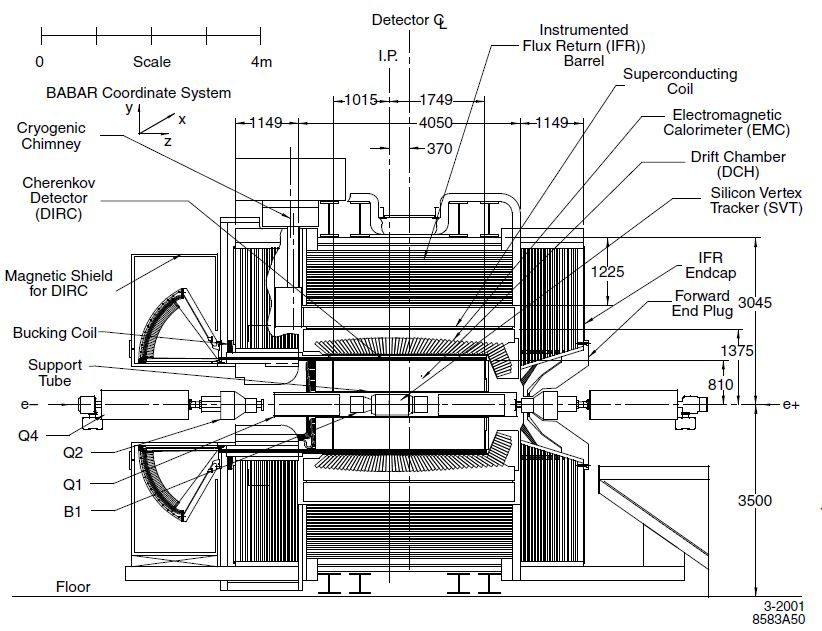
\includegraphics[width=0.75\textwidth]{figs/BBD.jpg}
\caption{The BaBar Detector Schematics}
\label{BBDa}
\end{figure}



%[working of C.o.M energy ~10.58GeV]

At 10.58GeV it is capable of producing an $\Upsilon(4s)$ which quickly decays to either a $B^+B^-$ or $B^0\overline{B}^0$ pair. Since the Upsilion rest mass is only just enough to create the pair the asymmetric energy beam provides the momentum to separate the pair, \cref{BBD}.
The uniqueness of this imbalance in momentum gives B mesons additional momentum upon creation relative to the laboratory center of mass frame. The benefit is that the distances the B mesons travel are then measurable and, due to time dilation induced by their high velocity, the lifetime of the B and $\overline{B}$ mesons can be determined and compared with considerable accuracy. The calculable separation that the Bs travel are on average 260um. The Upsilon's decays to the $B^0 \overline{B}^0$ pair a quarter of the time, which by that is a quarter of the total hadronic cross section [citation+decay table]. Thus the luminosity of the beam needs to be significantly high to have a reliable quantity of data.
The detector itself is the heart of the experiment and where some marvelous engineering and physics has been implemented to preform a detailed study of very specific decays with incredible high fidelity. The $\Upsilon(4s)$ is produced at the interaction point as shown in \cref{BBDa}. The decay products are sweep through the detector via their own momentum or under the influence of the 1.5T magnetic field produced by the superconducting coils \cite{B5}. 

\begin{figure}[h]
\centering
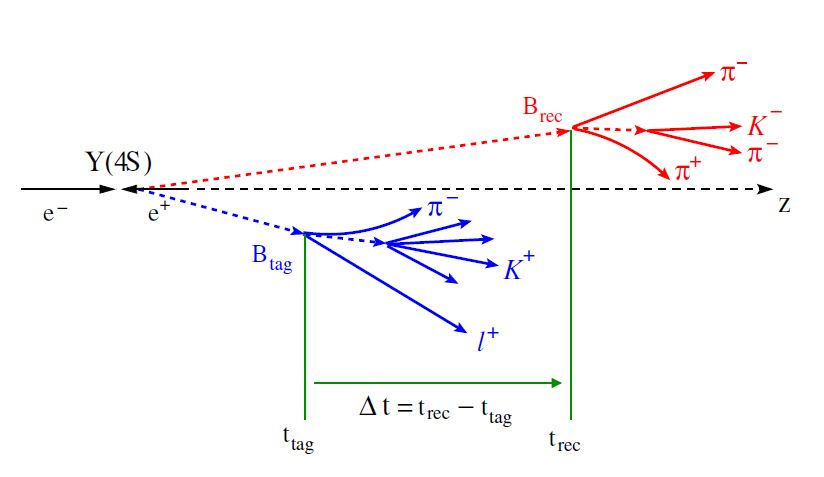
\includegraphics[width=0.75\textwidth]{figs/dt.JPG}
\caption{$\Upsilon (4s)$ decay illustrating the crucial experimental parameter $\Delta t$}
\label{BBD}
\end{figure}


\begin{itemize}
\item The Silicon Vertex Tracker(SVT) consists of five-layers of double sided silicon orientated as interlacing wafers along the inner most part of the detector. Residing only 3.2cm from the center of the 2.7cm radius beam pipe it receives  high fidelity detention of high energy charged particles and low energy $e^{+}$ $e^{-}$ pairs to an resolution of 10 microns \cite{B14}. The primarily purpose is to contribute to the measurement of the angular and vertex information (the z  and r - $\phi$)of each track which corresponds to the $\Delta z$ resolution where the z-axis is the parallel to the beam. The design had taken into consideration the asymmetric beam energy with the length of each layer increasing relative to the $x-y$ plane and shifted further down the z axis (along the higher energy beam path). Another design consideration to put in place was the radiation protection. Given the high luminosity of the beam and higher probability of Coulomb scattering inside the pipe the electronic were made to withstand the near $250kRad$ per year.


%[a1]http://hep.ucsb.edu/people/claudio/Vancouver.pdf
%[a2]http://www.slac.stanford.edu/cgi-wrap/getdoc/slac-pub-11695.pdfm


\item The Drift Chamber(DC) is responsible for measurements of the momentum of produced particles as well as information on identifying particles that lose energy inside (the value of $dE/dt$). It extends from the edge of the SVT (22cm) to a radial distance of 80cm . Inside are 7104 small cells connected to tungsten-rhenium sense wires. These wires have a 2kV potential across them and are thick enough to detect the ionized particles while keeping scattering minimal . The chamber contains a gas mixture of 20$\%$ Isobutane and 80$\%$ Helium allowing the atoms to be ionized and detected by the sense wires. \cite{B13}


%http://www.phys.hawaii.edu/superb04/talks/Kelsey.pdf


\item The Detector of Internally Reflected Cerenkov light (DIRC) takes advantage of the Cerenkov radiation. This is a process whereby charged particle traveling at speeds greater than the local speed of light in a medium. Silica rods are placed parallel to the beam pipe surround the outer wall of the Drift chamber. The large index of refraction ($n= 1.474$) means that the speed of light in that medium is only $0.68c$ and has a critical angle of about $43^{\circ}$. As charged particles enter the the silica rod and are of sufficient velocity they produce Cerenkov radiation and if it happens to be inside the critical angle it will be internally reflected along the rod to the back of the detector where they enter the ``standoff box" containing water and then detected by a ring (correctly speaking a toroidal) of Photomultiplier. Reflecting ``light catching cones" capture the light that might otherwise miss the PMT's active surface.  The energy and incident angle of each photon is reconstructed during analysis. The primary reason to have a system as such installed is to determine between Kaons and Pions between 0.5 and 4.5$GeV$, this is part of the particle Identification (PID) system. 


%[a3]http://www.slac.stanford.edu/cgi-wrap/getdoc/slac-pub-8080.pdf
\item The EM Calorimeter's (EMC) purpose is to measure the energy and angular resolution between 20 MeV and 9 GeV. The high energy bar provides detection of the more energetic electrons, muons and photon. Slow moving neutral particles such as the $\pi^0 \mbox{ and the } \eta^0$ will also be detected here. The particles rest mass energy is completely absorbed here due to interactions with the dense material. 6580 Csl(TI) (crystals grown from Csl and doped with 0.1$\%$ Thallium ) trapezoidal crystals are encased in carbon fiber modules .Each Crystal is roughly the dimensions of a standard Rubix cube. Physically it extends a 0.92m to 1.27m and parallel to the pipe 2.3m downstream and 1.5m upstream from the 9GeV beam. At the longer arm length there is an endcap of crystals to facilitate the off vertical production of end products. Moreover each module is angle towards the central interaction point \cite{B15}.

%http://iopscience.iop.org/1742-6596/160/1/012004/pdf/1742-6596_160_1_012004.pdf
\item The Instrument Flux Return (IFR) is separated from the EM Calorimeter by the superconducting coil and the farthest detection instrument from the Interaction point. Here muons and neutral hadrons (from the light $\pi^0$ to the heavy $K^{0}_{L}$ are detected with the use of the large iron structure needed as the magnetic return yoke. It is segmented into 19 hexagonal layers from 1.8m to 3m from the beam pipe. Between each layer is a single gap resistive plate chamber (RPC) which serves the purpose of detecting ionizing particles such as muon. Muons themselves are identified on the criterion of penetrating ever layer of iron, some slower muons are identified in the RPCs. 
\end{itemize}
%http://www.slac.stanford.edu/cgi-wrap/getdoc/slac-r-457.pdf
A process of particle Reconstruction and recognition from electronic signatures produced in the detector to the vast system of filtering and discriminating between background process using algorithms and triggering reveals the results to compare to theory. The time difference $\Delta t = \frac{\Delta z}{\left< \beta\gamma\right>} c$ is obtained from the measured $\Delta z=z_1 - z_2$ and average boost $\left<\beta\gamma\right>$ due to beam asymmetry. Since the boost is known to good precision, the $\Delta z$ measurement dominates over the $\Delta t$ resolution \cite{B4}.
\subsection{Experimental Evidence of \textit{CPV} in B mesons}
Testing B meson oscillations in the BaBar detector has been accomplished through the di-lepton and semi-leptonic events. An example of such a decay is $B^{0}\rightarrow D^{*-}l^{+}\nu$. By registering charged leptons the flavor of the decayed B meson can be calculated. Data taken at BaBar are plotted to a likelihood fit. The likelihood fit takes into account the probability of mismatched tags, the resolution of $\Delta t$ and background. In \cref{BBD4}.a the unmixed decays are shown where the B meson pair are of opposite flavor while B meson pairs that have identical flavors. The mixed state are found in \cref{BBD4}.b. Finally the time dependent asymmetry of the two is found in \cref{BBD4}.c clearly exhibiting a cosine wave form as predicted, almost akin to an inference pattern an undergraduate might observe in laboratories \cite{B19}. The frequency of the B meson oscillations is 80 GHz .\cite{B1}. Noticeably the amplitude of the Mixed state is significantly lower than unmixed. The neutral mixing frequency has been measure to high accuracy at BaBar, the inclusive dilepton sample was found to be $\Delta m_d = 0.493 \pm 0.012(stat) \pm 0.009(syst) ps^{-1}$.

 \begin{figure}[h]
\centering
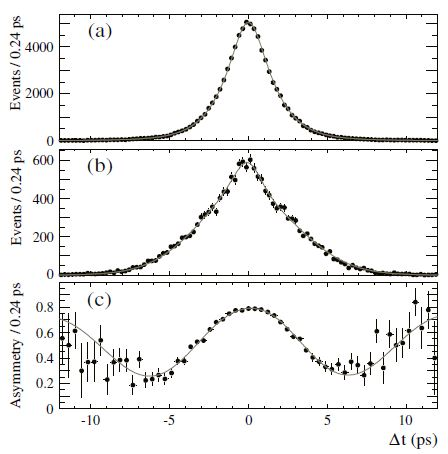
\includegraphics[width=0.5\textwidth]{figs/Flavourosscilatons.JPG}
\caption{(a) Unmixed flavored time dependent decay rate (b) Mixed flavored time dependent decay rate (c) Asymmetry of mixing in flavor eigenstates \cite{B1}}
\label{BBD4}
\end{figure}

The CP eigenstate decay is one of the most important measurements studied. Much of the theory on CKM matrixes are easily verified by these means. It can be approximated \cite{B2} that the amplitude in Eqn.(\ref{BPME19}) can be something like,
\begin{equation}\label{BPME20}
\frac{q}{p}\frac{\bar{A}_{f_{CP}}}{A_{f_{CP}}}=\eta_{f_{CP}}e^{2i\beta}, \left|\frac{q}{p}\frac{\bar{A}_{f_{CP}}}{A_{f_{CP}}}\right|=1, \it{I}m\frac{q}{p}\frac{\bar{A}_{f_{CP}}}{A_{f_{CP}}}=-\eta_{f_{CP}}\sin2\beta
\end{equation}
\begin{equation}\label{BPME21}
A_{CP}=-\eta_{f_{CP}}\sin2\beta\sin(\Delta m_d \Delta t)
\end{equation}
To obtain a value for the $\beta $ term we focus on two elements. The $\Delta t$ becomes important and allow for precision measurements of the asymmetry. The decay of interest here is $B\rightarrow J/\Upsilon K$, this is a favorable decay due to the large branching fractions $(\sim 10^{-4})$ and narrow resonance allowing a clean signal above background.\cite{B3}. In \ref{BBD5} the asymmetry manifesting due to CP violation is clearly visible with the data and likelihood fit corresponding to the predicted characteristics. The result for this is $\sin (2\beta) =0.722\pm 0.040_{stat} \pm0.023_{syst}$. Moreover due to ambiguities in the angle $\beta$  and further time depend analysis on the angular decay, $\cos(2\beta)$ is determined. The conclusion was that this is in agreement with the standard model\cite{B8}\cite{B16}.

 \begin{figure}[h]
\centering
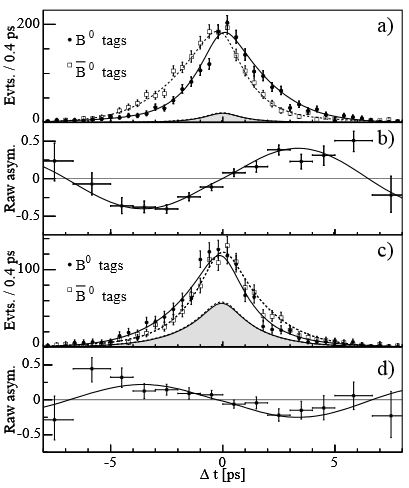
\includegraphics[width=0.36\textwidth]{figs/cpf.JPG}
\caption{(a) Time Distribution in CP odd, $K_{S}$ (b) Raw Asymmetry with likelihood plot for CP odd (c) Time Distribution in CP even, $K_{L}$  (d) Raw Asymmetry with likelihood plot for CP even \cite{B9}}
\label{BBD5}
\end{figure}

%\[\left| \frac{\bar{A}_{\bar{f}}} {A_{f}} \right|\neq 1 \]
%\[A_{CP}=\frac{1-\left|\frac{\bar{A}_{\bar{f}}}{A_f}\right|^2}{1+\left|\frac{\bar{A}_{\bar{f}}}{A_f}\right|^2}\neq 2\]
Since the $\beta$ angle has been determined one may now look towards finding a relevant $\gamma$ term to complete the unitary triangle. The CKM phase arises from the $V_{ub}$ term in the interferences of $b\rightarrow c \mbox{ and } b \rightarrow u$ transitions, note that the $V_{cb}$ term is phase-less. We construct six possible Feynman diagrams for this process,
\begin{equation}\label{BPME22}
B^0 \rightarrow D^{*\mp}\pi^{\pm} or B^0 \rightarrow D^{*\mp}\rho^{\pm} 
\end{equation}
The first two are seen in \cref{pBGD}. The charged products are clean pointers to a flavor of the $B_{rec}$ meson and it can infer the $B_{tag}$ flavor. As per the methods used in deriving Eqn.(\ref{BPME6}) and constructing the CP asymmetry term, in terms of j, where j is only a permutation between the various end products of decay.
\begin{equation}\label{BPME23}
\it{A}^{j}_{\it{CP}}(\Delta t) = \frac{2r^j}{1+\left[r^j\right]^2}\sin(2 \beta +\gamma)cos(\delta^j)\sin(\Delta m_d \Delta t)
\end{equation}
Since the decay \cite{B7} from $\bar{B}^0 \rightarrow D^{*+}\pi^{-}$, as in \cref{poBGD}, is favored via CKM mixing amplitudes over what is called the double-CKM-suppressed decay $B^0 \rightarrow D^{*+}\pi^{-}$ due to two low amplitude mixing terms there is a high sensitivity to the CP angle $\gamma$, \cref{kino1} is plot and a likelihood fit overlays the decay distribution. Since measurements of $\gamma$ are still in their infancy the present value is $\gamma = 78^{\circ}\pm12^{\circ}$. A discussion can be ignored on obtaining a value for $\alpha$ since no direct measurement have been successfully made, as no b quark transitions will produce such a phase. But it is possible to find a value intrinsically by the relations $\sin2\alpha = - \sin(2\beta +2\gamma)$ .\cite{B17} .

%http://cds.cern.ch/record/1106345/files/CERN-THESIS-2008-044.pdf
%MA BAAK thesis/paper
 \begin{figure}[h]
\centering
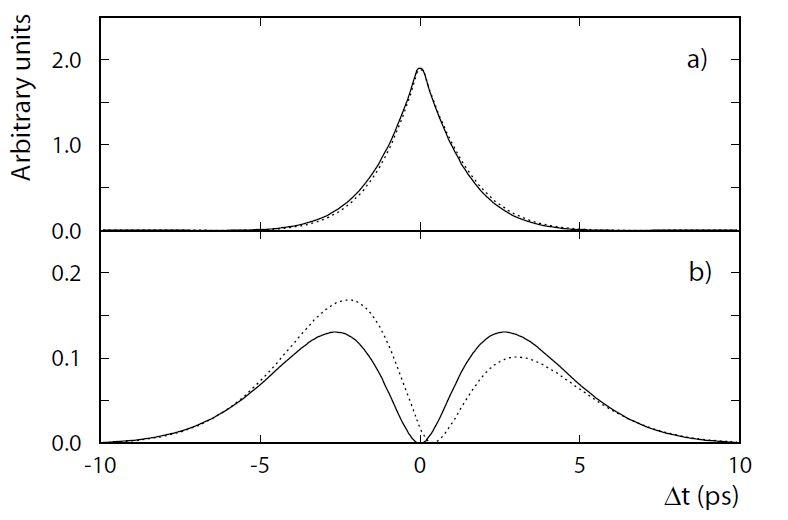
\includegraphics[width=0.6\textwidth]{figs/kino.JPG}
\caption{(a) Time dependent decay for $\bar{B}^0 \rightarrow D^{*-}\pi^{+}$ (b) Time dependent decay for $B^0 \rightarrow D^{*+}\pi^{-}$. If no double-CKM suppression were evident the dashed line would be the amplitude.}
\label{kino1}
\end{figure}

 \begin{figure}[h]
\centering
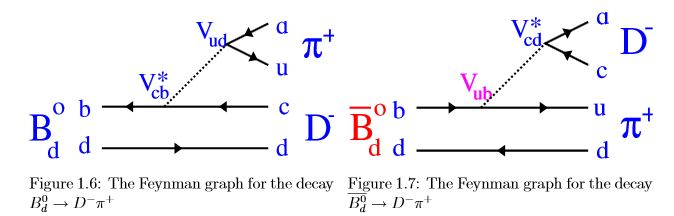
\includegraphics[width=0.8\textwidth]{figs/gam.JPG}
\caption{(a)$ B^{0} \rightarrow D^{-}\pi^{+}$ and $(b) \bar{B}^{0} \rightarrow D^{-}\pi^{+}$}
\label{poBGD}
\end{figure}


What has been demonstrated above are the consequences of three types of CP violation. Direct being the spontaneous decay via a CP operation. Indirect being a pure asymmetry in the mixing of B-states and the combination of the spontaneous and mixing. Of these there purely indirect has never been observed as the affects are minuscule and dominated in region of high background.
\\

The full range of angle measurement obtainable by B meson decay are shown in \cref{BBD9} .Remarkably the validation of this particular Unitary triangle has stood up to the rigorous measurements made at BaBar. It has paved a path for the further development of new physics to provide a concrete mechanism of interactions that may lead to a fundamental understanding of this asymmetry .\cite{B18}.
 \begin{figure}[h]
\centering
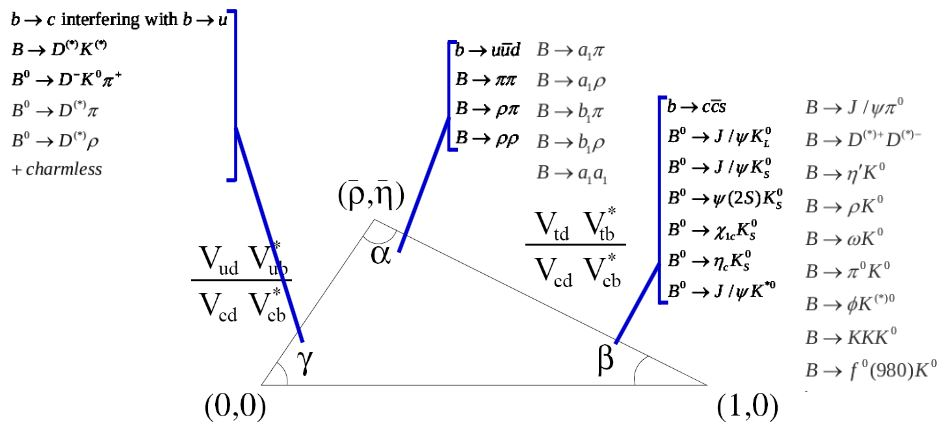
\includegraphics[width=0.8\textwidth]{figs/trig.JPG}
\caption{The B meson Unitary triangle}
\label{BBD9}
\end{figure}

%http://pprc.qmul.ac.uk/~bona/ulpg/cpv/lecture3.pdf


%\end{document}
